\pagebreak

\section{Procesos}
\begin{itemize}
    \item Programa en ejecución.
    \item \textbf{Programa:}
        \begin{itemize}
            \item Es estático.
            \item No tiene contador de programa.
            \item Existe desde que se edita hasta que se borra.
        \end{itemize}
    \item \textbf{Proceso:}
        \begin{itemize}
            \item Es dinámico.
            \item Tiene contador de programa.
            \item Su ciclo de vida comprende desde que se solicita ejecutar hasta que termina.
        \end{itemize}
\end{itemize}

\subsection{Atributos de un proceso}
\begin{itemize}
    \item Identificación del proceso y del proceso padre.
    \item Identificación del usuario que lo disparó.
    \item Si hay estructura de grupos, grupo que lo disparó.
    \item En ambientes multiusuario, desde qué terminal y quién lo ejecutó.
\end{itemize}

\subsection{Componentes de un proceso}
\begin{itemize}
    \item Sección de código.
    \item Sección de Datos.
    \item Stack(s): Datos temporarios.
\end{itemize}

\subsection{Process Control Block (PCB)}
\begin{itemize}
    \item Estructura de datos asociada al proceso (abstracción).
    \item Existe una por proceso.
    \item Es lo primero que se crea cuando se crea un proceso y lo último que se borra cuando termina.
    \item Contiene la información asociada con cada proceso:
        \begin{itemize}
            \item PID, PPID, etc.
            \item Valores de los registros de la CPU.
            \item Planificación.
            \item Ubicación en memoria.
            \item Accounting.
            \item Entrada/Salida.
        \end{itemize}
\end{itemize}

\subsubsection{Stacks}
\begin{itemize}
    \item Un proceso cuenta con 1 o más stacks.
    \item Se crean automáticamente y su medida se ajusta en run-time.
    \item Está formado por stack frames que son pushed (al llamar una rutina) y popped (cuando se retorna de ella).
    \item El stack frame tiene los parámetros de la rutina y los datos necesarios para recuperar el stack frame anterior.
\end{itemize}

\subsection{Espacio de direcciones de un proceso}
\begin{itemize}
    \item Conjunto de direcciones de memoria que ocupa el proceso.
    \item No incluye su PCB o tablas asociadas.
    \item Un proceso en modo usuario solo puede acceder a su espacio de direcciones.
    \item En modo Kernel, se puede acceder a estructuras internas (PCB del proceso) o a espacio de direcciones de otros procesos.
\end{itemize}
\begin{figure}[ht]
    \begin{center}
        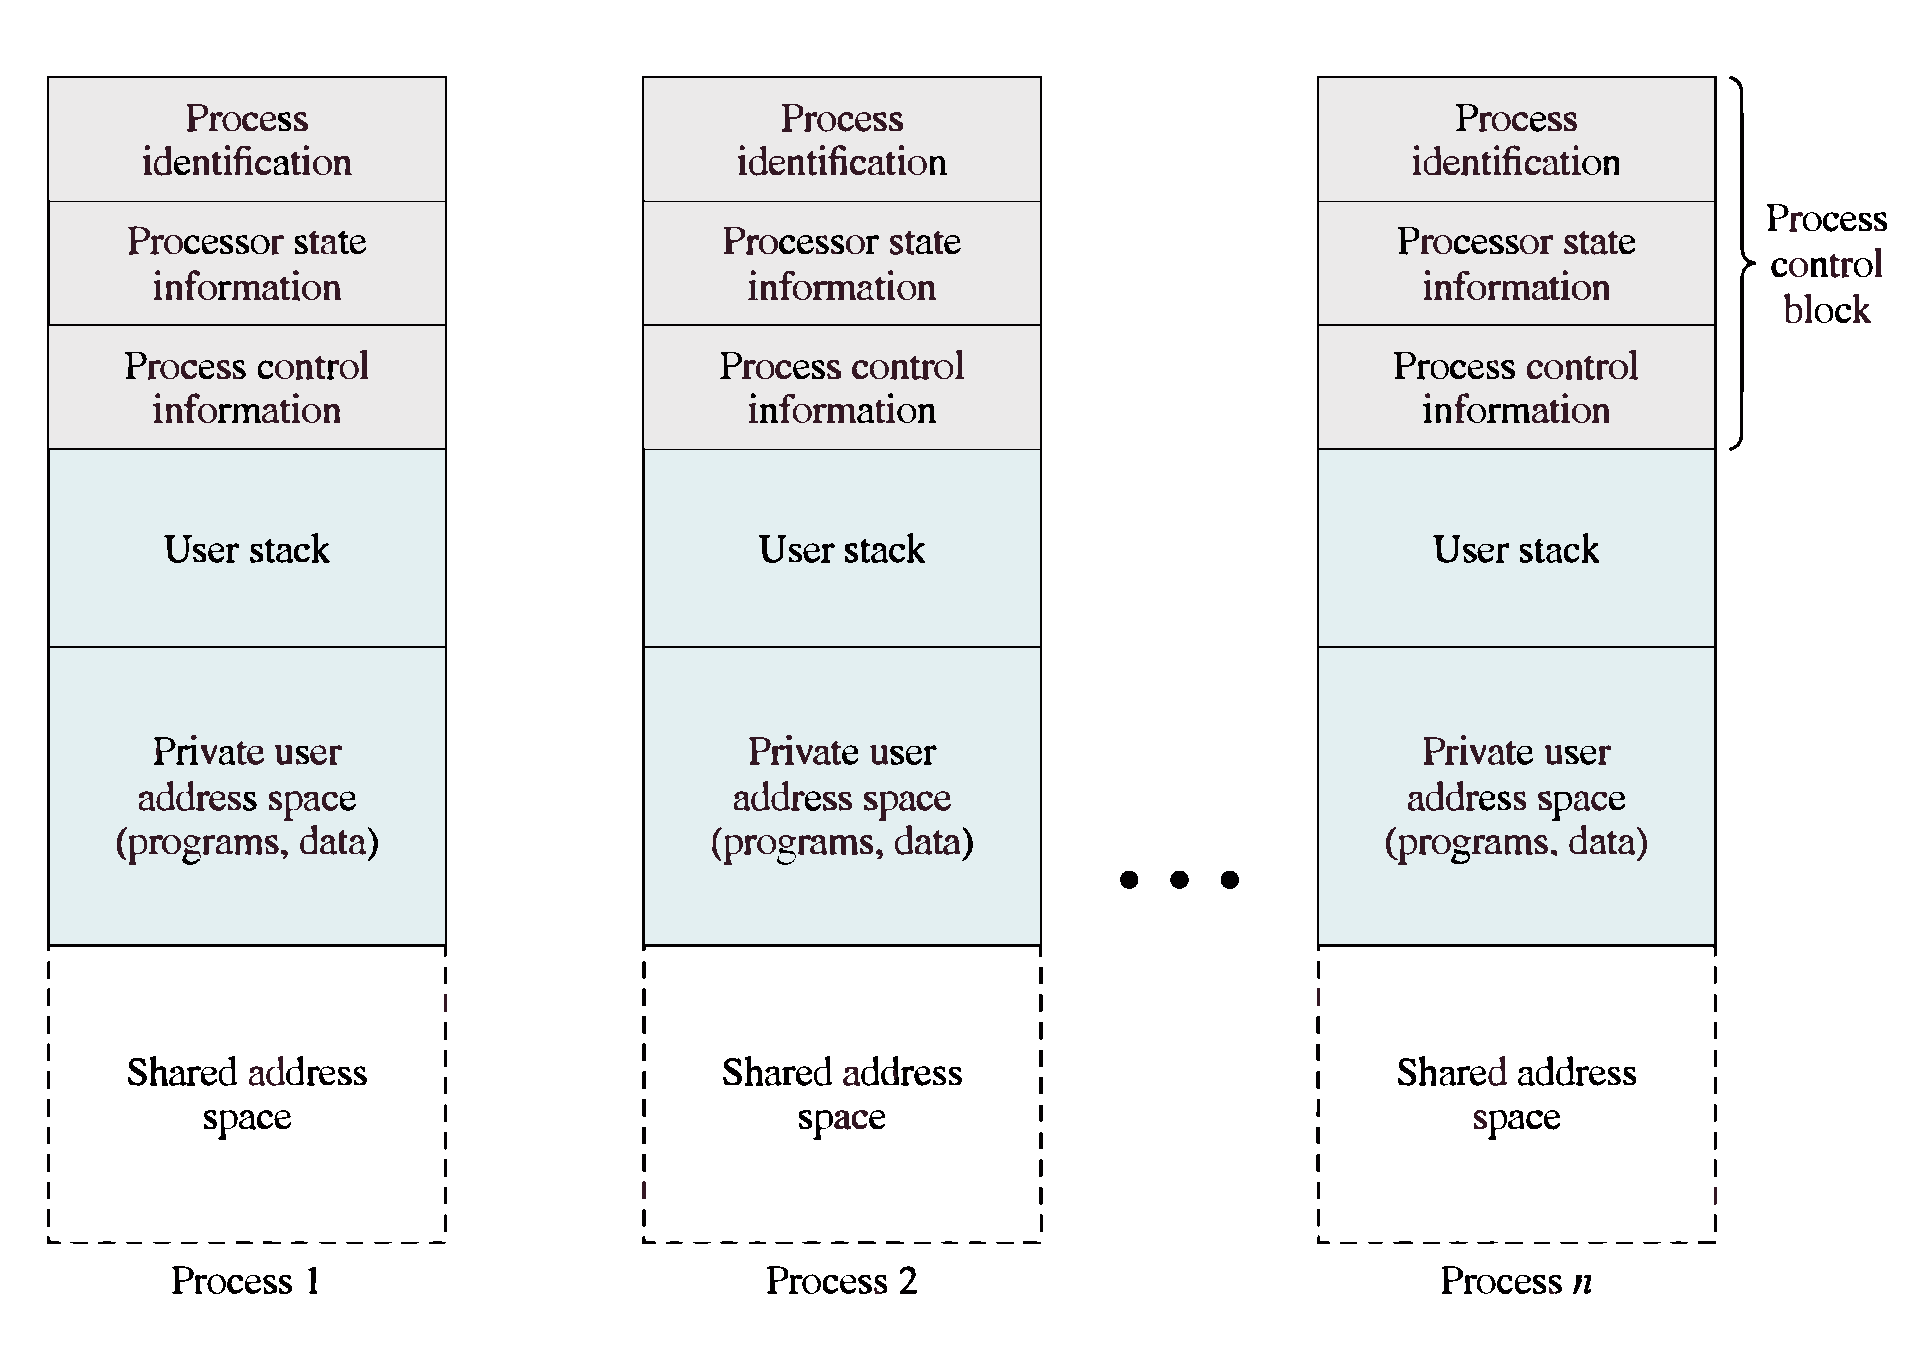
\includegraphics[width=0.90\textwidth]{assets/Proceso.eps}
    \end{center}
    \caption{Procesos en Memoria Virtual}\label{fig:1}
\end{figure}
\pagebreak

\subsection{Contexto de un proceso}
\begin{itemize}
    \item Incluye toda la información que el SO necesita para administrar el proceso, y la CPU para ejecutarlo correctamente.
    \item Son parte del contexto, los registros de CPU, inclusive el contador del programa, prioridad, etc.
\end{itemize}
\subsubsection{Context Switch}
\begin{itemize}
    \item Se produce cuando la CPU cambia de un proceso a otro.
    \item Se debe resguardar el contexto del proceso saliente, que pasa a espera y retornará después a la CPU.
    \item Se debe cargar el contexto del nuevo proceso y comenzar desde la instrucción siguiente a la última ejecutada en dicho contexto.
    \item Es tiempo no productivo de la CPU.
    \item El tiempo que consume depende del soporte de HW.
\end{itemize}
\begin{figure}[ht]
    \begin{center}
        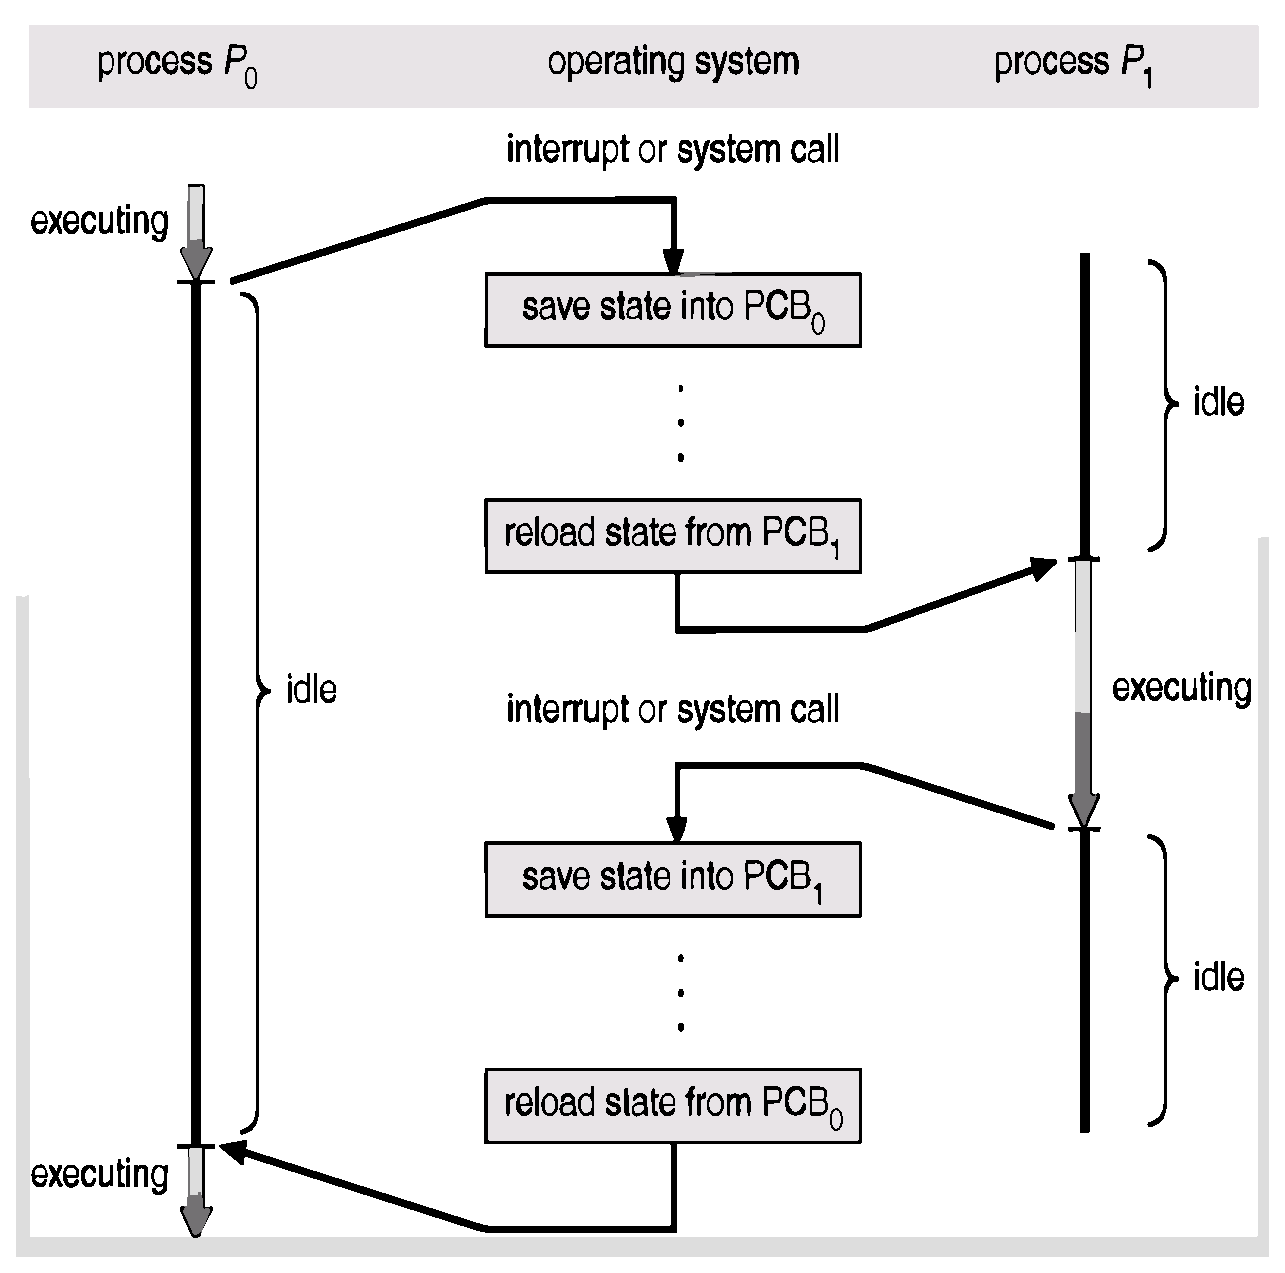
\includegraphics[width=0.65\textwidth]{assets/ContextSwitch.eps}
    \end{center}
    \caption{Context Switch}\label{fig:}
\end{figure}

\subsection{Ejecución del Kernel}
\begin{itemize}
    \item El kernel es un conjunto de módulos de software.
    \item Se ejecuta en el procesador como cualquier otro proceso.
    \item Existen diferentes enfoques de diseño:
\end{itemize}
\subsubsection{El kernel como entidad independiente}
\begin{itemize}
    \item El kernel se ejecuta fuera de todo proceso.
    \item Cuando un proceso es interrumpido o realiza una System Call, el contexto del proceso se salva y el control se pasa al Kernel del SO.
    \item El kernel posee su propia región de memoria y su propio Stack.
    \item Finalizada su actividad, le devuelve el control al proceso.
    \item El kernel NO es un proceso.
    \item Se ejecuta como una entidad independiente en modo privilegiado.
\end{itemize}
\begin{figure}[h]
    \begin{center}
        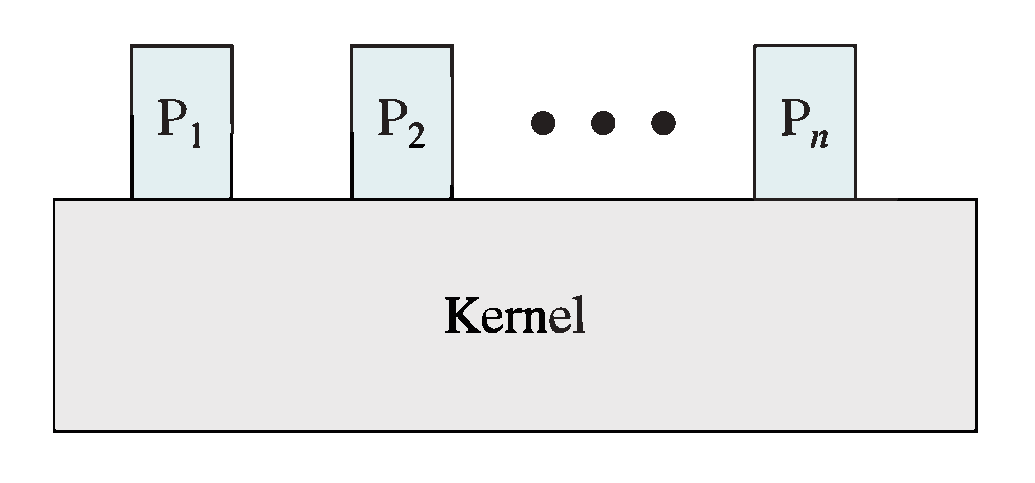
\includegraphics[width=0.45\textwidth]{assets/Kernel1.eps}
    \end{center}
    \caption{Kernel como entidad independiente}\label{fig:}
\end{figure}

\vspace{2cm}

\subsubsection{El kernel "dentro" del proceso}
\begin{itemize}
    \item El código del Kernel se encuentra dentro del espacio de direcciones de cada proceso.
    \item El Kernel se ejecuta en el mismo contexto que algún proceso de usuario.
    \item El Kernel se puede ver como una colección de rutinas que el proceso utiliza.
    \item Dentro de un proceso se encuentra el código del programa y el código de los módulos SW del SO (kernel).
    \item Cada proceso tiene un stack en modo usuario y otro en modo Kernel. 
    \item Cada interrupción es atendida en el contexto del proceso que se encontraba en ejecución (en modo kernel).
    \item Si el SO determina que el proceso debe seguir ejecutándose luego de atender la interrupción, cambia a modo usuario y devuelve el control.
\end{itemize}
\vspace{1cm}
\begin{figure}[ht]
    \begin{center}
        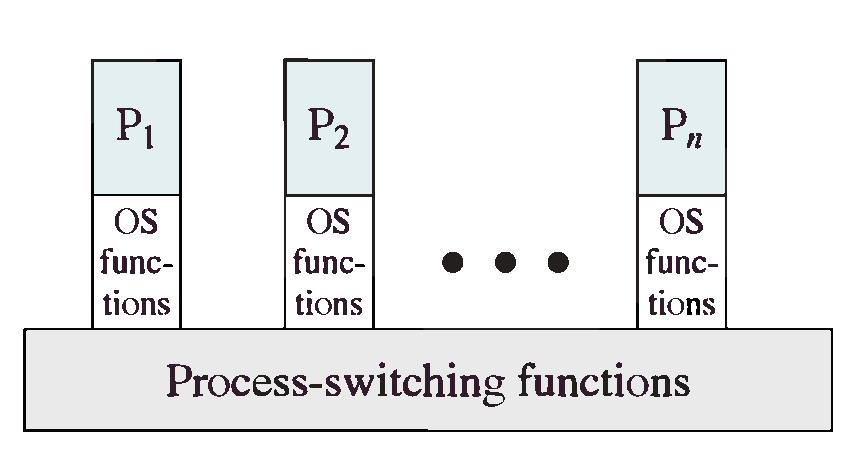
\includegraphics[width=0.50\textwidth]{assets/Kernel2.eps}
    \end{center}
    \caption{Kernel dentro del proceso}\label{fig:}
\end{figure}

\subsection{Estados de un Proceso}
En su estado de vida, un proceso pasa por diferentes estados:
\begin{itemize}
    \item \textbf{Nuevo (new)}.
    \item \textbf{Listo (ready)}.
    \item \textbf{Ejecución (running)}.
    \item \textbf{En espera/bloqueado (waiting/blocked)}.
    \item \textbf{Terminado (terminated)}.
\end{itemize}

\begin{figure}[h]
    \begin{center}
        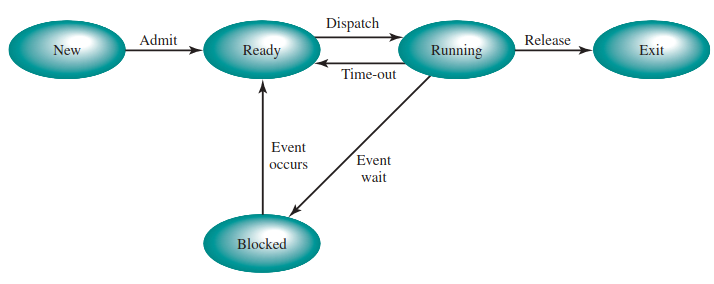
\includegraphics[width=0.90\textwidth]{assets/estados.png}
    \end{center}
    \caption{Estados de un proceso}\label{fig:}
\end{figure}


\subsection{Colas en la planificación de procesos}
\begin{itemize}
    \item Para realizar la planificación, el SO utiliza la PCB de cada proceso como una abstracción del mismo.
    \item Las PCB se enlazan en colas siguiendo un orden determinado.
\end{itemize}
\begin{figure}[h]
    \begin{center}
        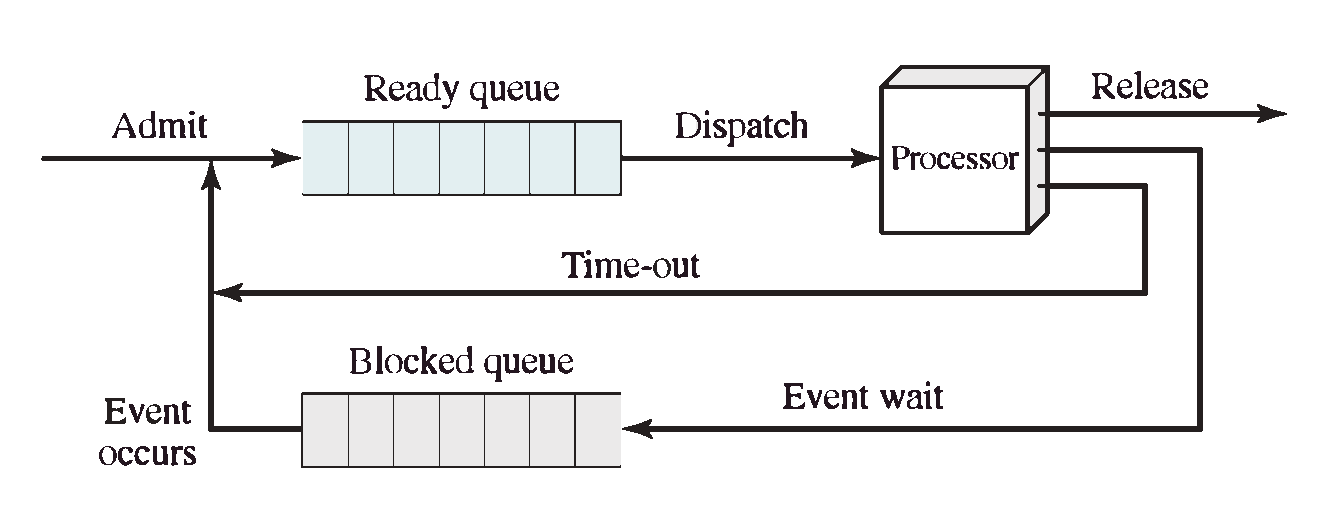
\includegraphics[width=0.75\textwidth]{assets/ProcessQueue.eps}
    \end{center}
    \caption{Colas de Planificación}\label{fig:}
\end{figure}
\pagebreak

\subsubsection{Módulos de la planificación}
\begin{itemize}
    \item Son módulos de SW del Kernel que realizan distintas tareas asociadas a la planificación.
    \item Se ejecutan ante determinados eventos:
    \begin{itemize}
        \item Creación/Terminación de procesos.
        \item Eventos de sincronización.
        \item Finalización de lapso de tiempo.
        \item Etc.
    \end{itemize}
    \item Existen 3 schedulers:
        \begin{itemize}
            \item \textbf{Long Term Scheduler} 
            \item \textbf{Short Term Scheduler} 
            \item \textbf{Medium Term Scheduler} 
        \end{itemize}
    \item \textbf{Dispatcher:} realiza el cambio de contexto, cambio de modo de ejecución y despacha el proceso elegido por el Short Term.
    \item \textbf{Loader} carga en memoria el proceso elegido por el long term.
\end{itemize}
\pagebreak
\begin{figure}[h]
    \begin{center}
        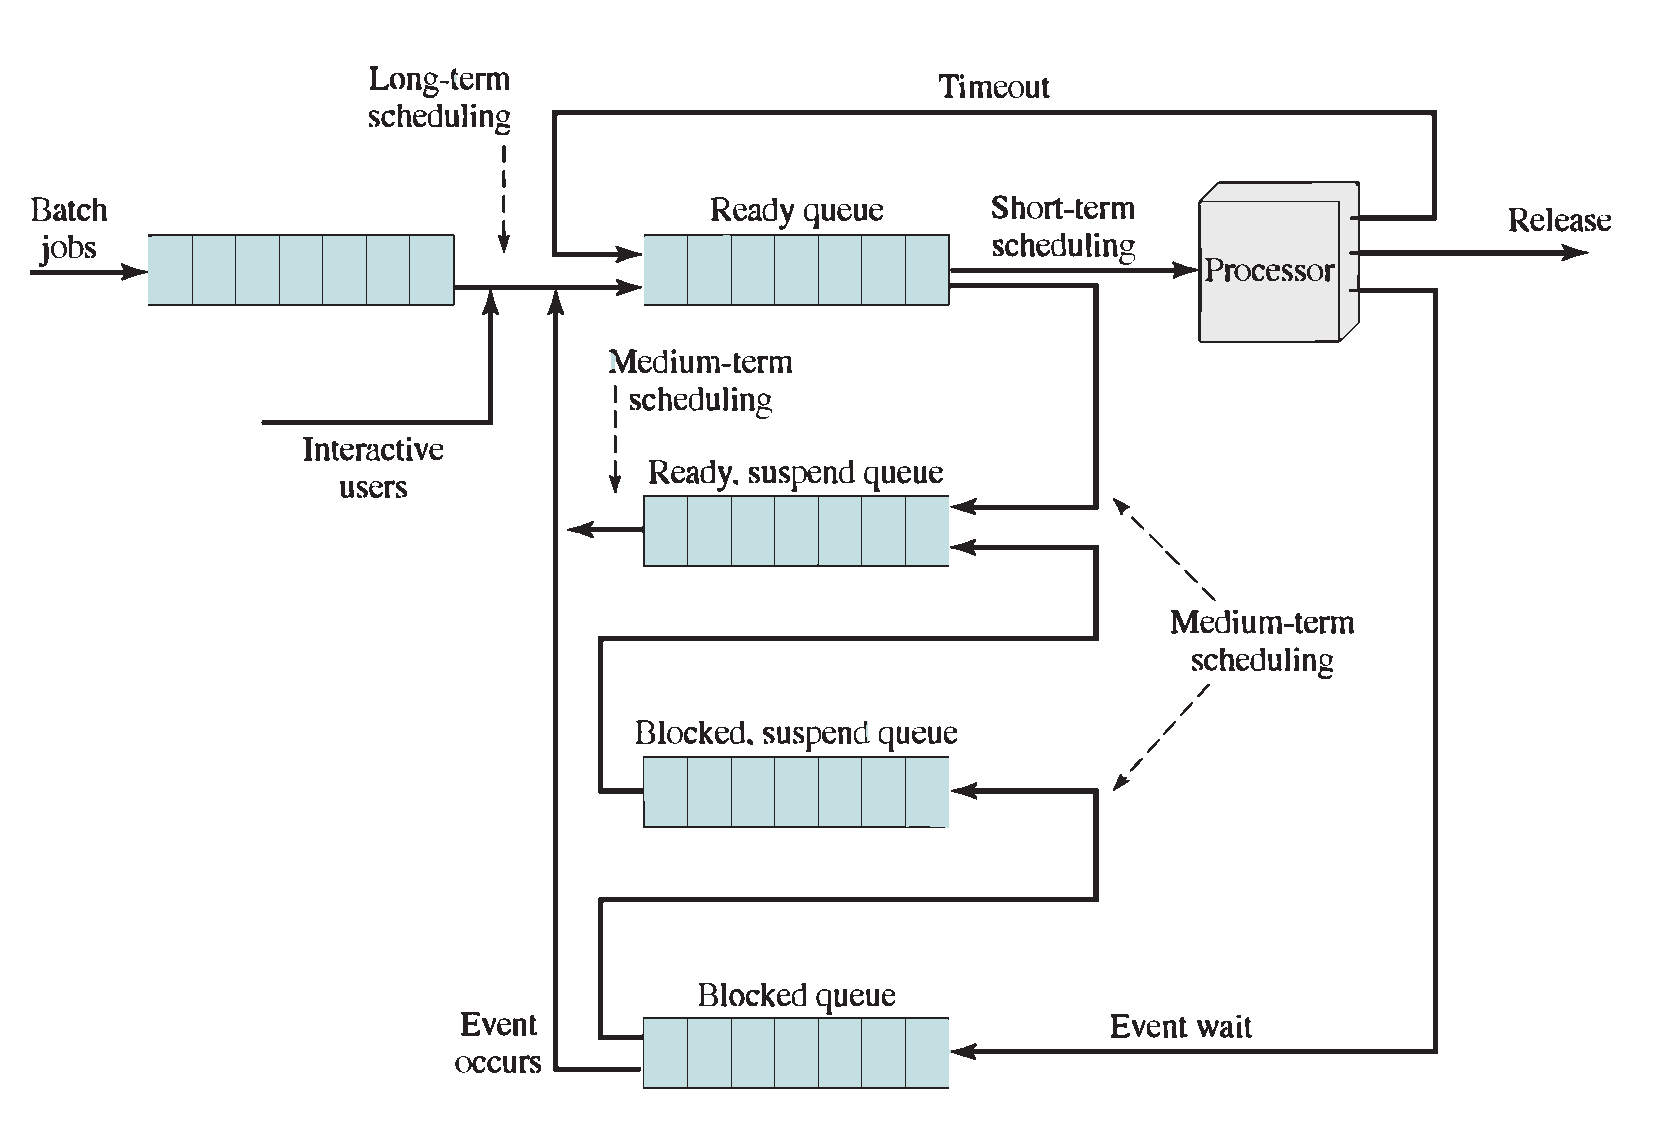
\includegraphics[width=0.90\textwidth]{assets/Schedulers.eps}
    \end{center}
    \caption{Funcionamiento de los Schedulers}\label{fig:}
\end{figure}


\subsubsection{Schedulers}
\begin{itemize}
    \item \textbf{Long Term Scheduler}
        \begin{itemize}
            \item Controla el grado de multiprogramación.
            \item Puede no existir este scheduler y absorber esta tarea el de short term.
        \end{itemize}
    \item \textbf{Medium Term Scheduler}
        \begin{itemize}
    \item Si es necesario, reduce el grado de multiprogramación.
    \item Saca temporalmente de memoria los procesos que sean necesarios para mantener el equilibrio del sistema.
\end{itemize}
\item \textbf{Short Term Scheduler}
\begin{itemize}
    \item Decide a cuál de los procesos en la cola de listos se elige para que use la CPU.
    \item Términos asociados: apropiativo, no apropiativo, algoritmo de scheduling.
\end{itemize}
\end{itemize}

\begin{figure}[ht]
    \begin{center}
        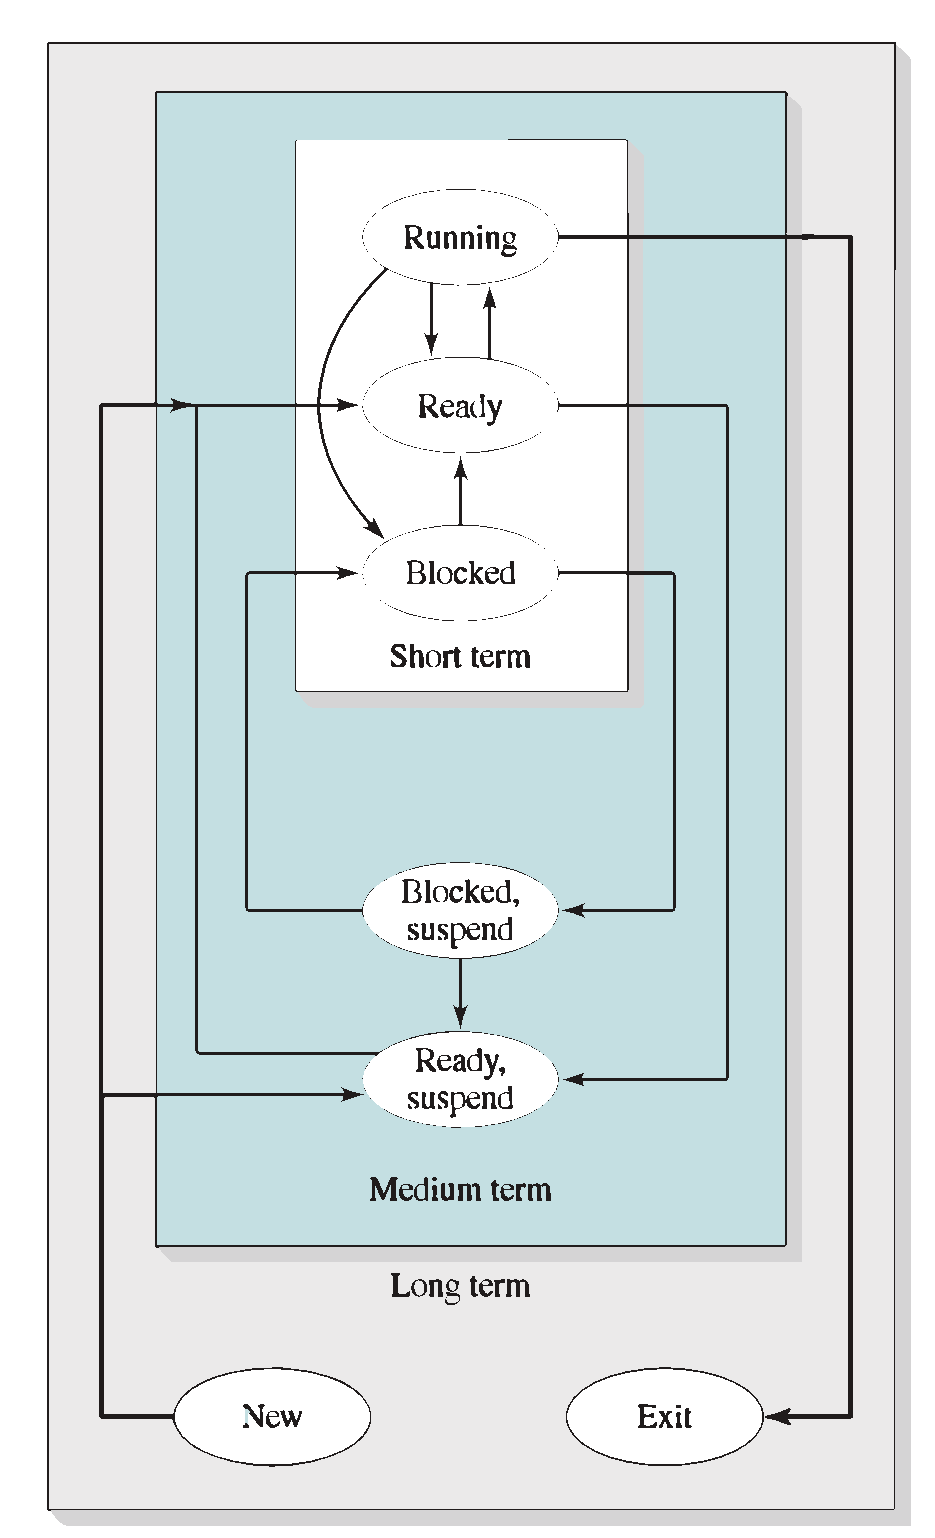
\includegraphics[width=0.50\textwidth]{assets/Schedulers2.pdf}
    \end{center}
    \caption{Schedulers}\label{fig:5}
\end{figure}

\subsection{Estados de los procesos}
\begin{itemize}
    \item \textbf{Nuevo (new):}
        \begin{itemize}
            \item Un usuario "dispara" el proceso. Un proceso es creado por otro proceso: su proceso padre.
            \item En este estado, se crean las estructuras asociadas, y el proceso queda en la cola de procesos, normalmente en espera de ser cargado en memoria.
        \end{itemize}
    \item \textbf{Listo (ready):}
        \begin{itemize}
            \item Luego de que el Long Term Scheduler elige al proceso para cargarlo en memoria, el proceso queda en estado listo.
            \item El proceso solo necesita que se le asigne CPU.
            \item Está en la cola de procesos listos (ready queue).
        \end{itemize}
    \item \textbf{Ejecución (running):}
        \begin{itemize}
            \item El Long Term Scheduler lo eligió para asignarle CPU.
            \item Tendrá la CPU hasta que se termine el período de tiempo asignado, termine o hasta que necesite realizar alguna operación de E/S.
        \end{itemize}
    \item \textbf{En espera/bloqueado (waiting/blocked):}
    \begin{itemize}
        \item El proceso necesita que se cumpla el evento esperado para continuar.
        \item El evento puede ser la terminación de una E/S solicitada, o la llegada de una señal por parte de otro proceso.
        \item Sigue en memoria, pero no tiene la CPU.
        \item Sigue en memoria, pero no tiene la CPU.
    \end{itemize}
\end{itemize}

\subsection{Comportamiento de los procesos}
\begin{itemize}
    \item \textbf{CPU-bound:} mayor parte del tiempo utilizando la CPU.
    \item \textbf{I/O bound:} mayor parte del tiempo esperando por I/O.
\end{itemize}

\subsection{Algoritmos de Planificación}
\begin{itemize}
    \item \textbf{Planificación:} necesidad de determinar cuál de todos los procesos que están listos para ejecutarse, será el próximo en ejecutarse.
    \item \textbf{Algoritmos Preemptive:} existen situaciones que hacen que el proceso en ejecución sea expulsado de la CPU.
    \item \textbf{Algoritmos No Preemptive:} los procesos se ejecutan hasta que el mismo (por su propia cuenta) abandone la CPU.
\end{itemize}

\subsection{Algoritmos según el tipo de proceso}
\subsubsection{Procesos Batch}
\begin{itemize}
    \item No existen usuarios que esperen una respuesta en la terminal.
    \item Se pueden utilizar algoritmos no apropiativos.
    \item Metas propias de este tipo de algoritmos:
        \begin{itemize}
            \item Rendimiento: Maximizar el número de trabajos por hora.
            \item Tiempo de Retorno: Minimizar los tiempos entre el comienzo y la finalización.
            \item El tiempo de espera se puede ver afectado.
            \item Uso de la CPU: Mantener la CPU ocupada la mayor cantidad de tiempo posible.
        \end{itemize}
\end{itemize}

\subsubsection{Procesos Interactivos}
\begin{itemize}
    \item No solo interacción con los usuarios.
    \item Son necesarios algoritmos apropiativos para evitar que un proceso acapare la CPU.
    \item Metas propias de este tipo de algoritmos:
    \begin{itemize}
        \item Tiempo de respuesta: Responder a peticiones con rapidez.
        \item Proporcionalidad: Cumplir con las expectativas de los usuarios. Por ejemplo, al poner STOP al reproductor de música, debe dejar de ser reproducida en un tiempo corto.
    \end{itemize}
\end{itemize}

\subsection{Creación de procesos}
\begin{itemize}
    \item Un proceso es creado por otro proceso.
    \item Un proceso padre tiene uno o más procesos hijos.
    \item Se forma un árbol de procesos.
    \item Actividades en la creación:
    \begin{itemize}
        \item Crear la PCB.
        \item Asignar PID único.
        \item Asignarle memoria para regiones.
        \item Crear estructuras de datos asociadas.
    \end{itemize}
\end{itemize}

\subsubsection{Relación entre procesos padre e hijo}
\begin{itemize}
    \item El padre puede continuar ejecutándose concurrentemente con su hijo.
    \item El padre puede esperar a que el/los procesos hijos terminen para continuar la ejecución.
\end{itemize}
